\newpage

\section[Day 7: Metric Spaces and Closed/Open]{ Metric Spaces \& Closed/Open }

\subsection{ Metric Spaces }

{ \color{blue} Definition 7.1.1: Metric Spaces } 

	\begin{adjustbox}{minipage=14cm, right, vspace=0.1cm 0cm}
		A set X is a metric space if for ant p,q $\in$ X, there is an associated d(p,q) $\in$
		$\mathbb{R}$ such that:	
		\begin{itemize}[leftmargin=1cm, itemsep=0.1cm]
			\item d(p,q) $>$ 0 \qquad \qquad if p $\neq$ q
			
			\item d(p,q) = 0 if and only if p = q
			
			\item {\color{lblue} Symmetry}:
				d(p,q) = d(q,p)
			
			\item {\color{lblue} Triangle Inequality}:
				d(p,q) $\leq$ d(p,r) + d(r,q) \qquad \qquad for any r $\in$ $\mathbb{R}$.
		\end{itemize}

		For euclidean spaces $\mathbb{R}^k$, d(x,y) = $| x - y |$ where x,y $\in$ $\mathbb{R}^k$. \\
	\end{adjustbox}

{ \color{blue} Definition 7.1.2: Types of Points and Sets } 
	\begin{enumerate}[label=(\alph*), leftmargin=2cm, itemsep=0.1cm]
		\item {\color{lblue} Neighborhood}

			\qquad For p $\in$ $\mathbb{R}^k$ and r $>$ 0, N$_r(p)$ is the set of all q $\in$ X
			where d(q,p) $<$ r

			\begin{figure}[h]
				\centering
				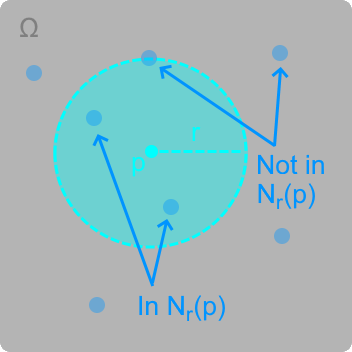
\includegraphics[scale=0.45]{Images/7.1.2a.png}
			\end{figure}

		\item {\color{lblue} Limit Points and Closed Sets}

			\hspace{0.1cm} Closed set E contain all p $\in$ X where every N$_r(p)$ contain
			a q $\neq$ p $\in$ E

			\begin{itemize}[leftmargin=1cm, itemsep=0.1cm]
				\item Limit Points 

					\qquad For point p $\in$ X, every N$_r(p)$ contains a
					q $\neq$ p $\in$ E
				
				\item Isolated Points

					\qquad If p $\in$ E is not a limit point of E

				\item Closed

					\qquad If every limit point p of E is a p $\in$ E
			\end{itemize}

			\begin{figure}[h]
				\centering
				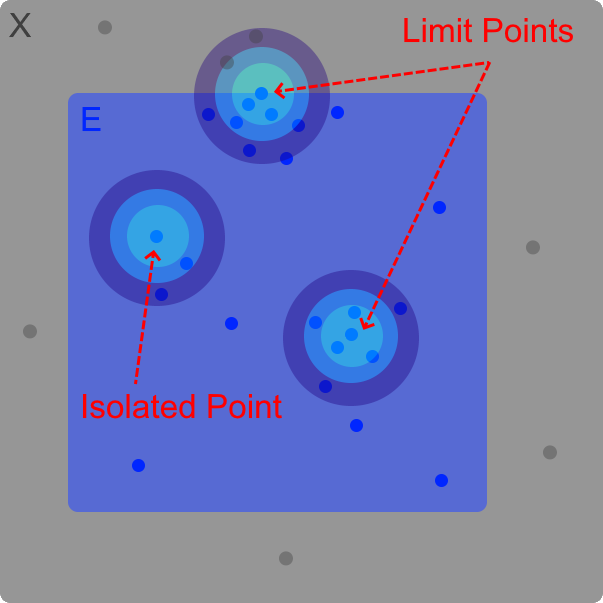
\includegraphics[scale=0.3]{Images/7.1.2b.png}
			\end{figure}

\newpage

		\item {\color{lblue} Interior Points and Open Sets}

			\hspace{0.1cm} Open set E contains all its p which has a N$_r(p)$ $\subset$ E
			
			\begin{itemize}[leftmargin=1cm, itemsep=0.1cm]
				\item Interior Point

					\qquad For p $\in$ X, there is a N$_r(p)$ $\subset$ E

				\item Open

					\qquad If every p $\in$ E is an interior point of E
			\end{itemize}

			\begin{figure}[h]
				\centering
				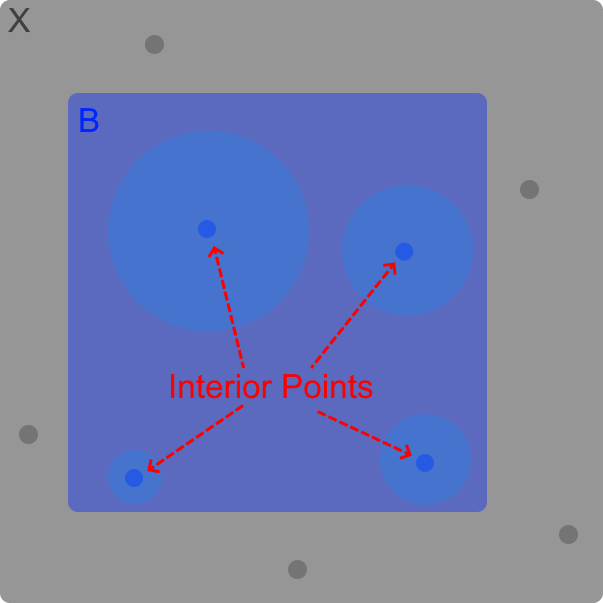
\includegraphics[scale=0.3]{Images/7.1.2c.png}
			\end{figure}

		\item {\color{lblue} More about Sets}
			
			\begin{itemize}[leftmargin=1cm, itemsep=0.1cm]
				\item Bounded

					\qquad If there is M $\in$ $\mathbb{R}$ , q $\in$ X such that d(p,q) $<$ M
					for all p $\in$ E

				\item Complement

					\qquad From E, E$^\text{c}$ is the set of all p $\in$ X such that p $\not \in$ E

				\item Perfect

					\qquad If E is closed and if every p $\in$ E is a limit point of E

				\item Dense

					\qquad If every p $\in$ X is a limit point of E or/and p $\in$ E \\
			\end{itemize}
	\end{enumerate}

	\qquad For a metric space X, X and $\emptyset$ are both open and closed. \\

{ \color{red} Theorem 7.1.3: N$_r(p)$ is open } 

	\begin{adjustbox}{minipage=14cm, right, vspace=0.1cm 0cm}
		Every neighborhood is an open set.
	\end{adjustbox}

{ \color{magenta} \underline{Proof} } 
	
	Let q $\in$ N$_r(p)$. Then there is a h $>$ 0 $\in$ $\mathbb{R}$
	such that d(q,p) = r - h.

	Then for any s $\in$ N$_h(q)$:

	\qquad d(s,p) $\leq$  d(s,q) + d(q,p) = h + (r - h) = r

	Thus, for any q $\in$ N$_r(p)$, there exists a N$_h(q)$ $\subset$ N$_r(p)$.

\begin{figure}[h]
	\centering
	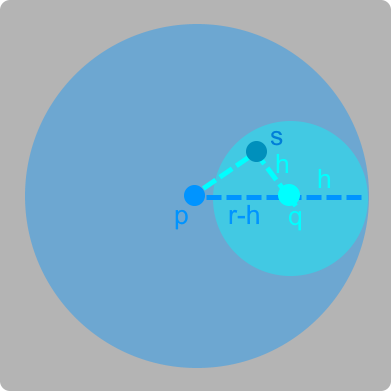
\includegraphics[scale=0.36]{Images/7.1.3.png}
\end{figure}

\newpage

{ \color{red} Theorem 7.1.4: If a set has a limit point, there are infinite q
$\in$ E in N$_r(p)$ } 
	
	\begin{adjustbox}{minipage=14cm, right, vspace=0.1cm 0cm}
		If p is a limit point of set E, then every N$_r(p)$ contains infinitely many q $\in$ E.
	\end{adjustbox}

{ \color{magenta} \underline{Proof} } 
	
	Suppose there is N$_{r_1}(p)$ which contains finitely many q = \{ q$_1$, ... , q$_n$ \}.

	Let r = min$_{m \in [1,n]}$ d(p,q$_m$). Then N$_r(p)$ contains no q $\in$ E such that q $\not =$ p.

	So, p is not a limit point of E which is a contradiction since p is a limit point of E.

\begin{figure}[h]
	\centering
	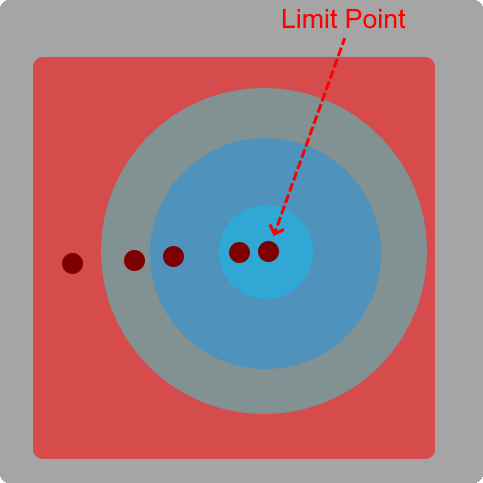
\includegraphics[scale=0.31]{Images/7.1.4.png}
\end{figure}

{ \color{orange} Corollary 7.1.5: Limit points do not exist in finite sets } 
	
	\begin{adjustbox}{minipage=14cm, right, vspace=0.1cm 0cm}
		A finite set E has no limit points.
		Since $\emptyset$ $\in$ A, all finite set must be closed.
	\end{adjustbox}

{ \color{magenta} \underline{Proof} } 

	Let p be a limit point of finite set E. By {\color{red} theorem 7.1.4}, 
	then any N$_r(p)$ contain infinite q $\in$ E so E is an infinite set
	which is a contradiction since E is finite.

	So p cannot be limit point of E and thus, E has no limit points. \\

{ \color{red} Theorem 7.1.6: De Morgan's Laws } 
	
	\begin{adjustbox}{minipage=14cm, right, vspace=0.1cm 0cm}
		Let $E_1, E_2 , ... $ be a collection of sets. Then,
		($\cup_{}^{}$ $E_x$)$^\text{c}$ = $\cap_{}^{}$ ($E_x$$^\text{c}$).
	\end{adjustbox}

{ \color{magenta} \underline{Proof} } 
	
	If p $\in$ ($\cup_{}^{}$ $E_x$)$^\text{c}$, then p $\not \in$ ($\cup_{}^{}$ $E_x$).

	Thus, p $\not \in$ $E_x$ for any x so p $\in$ E$_x^\text{c}$ for all x.
	Thus, p $\in$ $\cap_{}^{}$ ($E_x^c$) so
	($\cup_{}^{}$ $E_x$)$^c$ $\subset$ $\cap_{}^{}$ ($E_x^c$).

	If p $\in$ $\cap_{}^{}$ ($E_x^c$), then p $\in$ $E_x^c$ for all x.
	
	Thus, p $\not \in$ $E_x$ for any x so p $\not \in$ $\cup_{}^{}$ $E_x$.
	Thus, p $\in$ ($\cup_{}^{}$ $E_x$)$^c$ so
	$\cap_{}^{}$ ($E_x^c$) $\subset$ ($\cup_{}^{}$ $E_x$)$^c$.

	Thus, ($\cup_{}^{}$ $E_x$)$^c$ = $\cap_{}^{}$ ($E_x^c$). \\

\begin{figure}[h]
	\centering
	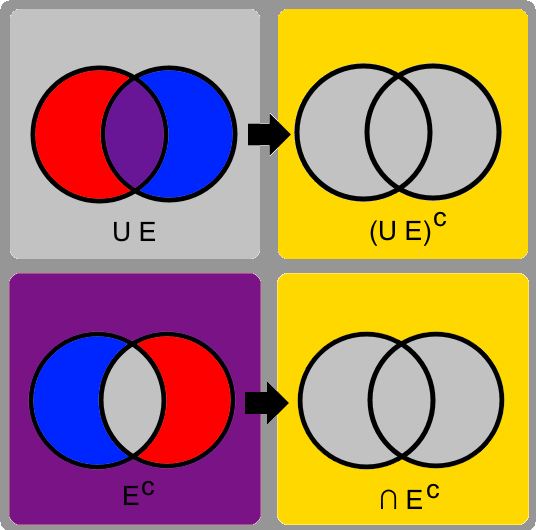
\includegraphics[scale=0.35]{Images/7.1.6.png}
\end{figure}

\newpage

{ \color{red} Theorem 7.1.7: Open set $\rightarrow$ Closed complement } 

	\begin{adjustbox}{minipage=14cm, right, vspace=0.1cm 0cm}
		A set E is open if and only if E$^\text{c}$ is closed.
	\end{adjustbox}

{ \color{magenta} \underline{Proof} } 

	Suppose E is open. Let x be a limit point of E$^c$.

	Then for every r $>$ 0, N$_r(x)$ must contain a p $\in$ E$^c$ such that p $\neq$ x.

	Then, N$_r(x)$ $\not \subset$ E so x is not an interior point of E and
	thus, x $\not \in$ E so x $\in$ E$^c$.

	Since any limit point x of E$^c$ is a x $\in$ E$^c$, then E$^c$ is closed.

	\vspace{0.2cm}

	Suppose E$^c$ is closed. Let x $\in$ E.

	Since x $\not \in$ E, x is not a limit point of E.

	Then there exists a r $>$ 0 such that any p $\in$ N$_r(x)$ is not in E.

	Thus, every p $\in$ N$_r(x)$ is p $\in$ E so N$_r(x)$ $\subset$ E and thus,
	x is an interior point of E.

	Since any x $\in$ E is an interior point of E, then E is open. \\

{ \color{orange} Corollary 7.1.8: Closed set $\rightarrow$ Open complement } 

	\begin{adjustbox}{minipage=14cm, right, vspace=0.1cm 0cm}
		A set F is closed if only only if F$^\text{c}$ is open.
	\end{adjustbox}

{ \color{magenta} \underline{Proof} } 

	From {\color{red} theorem 7.1.7}, let E = F$^\text{c}$. \\

{ \color{red} Theorem 7.1.9: Union open $\rightarrow$ open and
Intersection closed $\rightarrow$ closed } 

	\begin{enumerate}[label=(\alph*), leftmargin=2cm, itemsep=0.4em]
		\item If $\{G_x\}$ is a finite or infinite collection of open sets,
		then $\cup$ $G_x$ is open.

			{ \color{magenta} \underline{Proof} }

				If p $\in$ $\cup$ $G_x$, then p $\in$ $G_x$ for at least one x.
				Let $\overline{x}$ be such an x.

				Since $G_{\overline{x}}$ is open, then p is an interior point of
				$G_{\overline{x}}$ and thus, there is a N$_r(p)$ such that
				N$_r(p)$ $\subset$ $G_{\overline{x}}$ $\subset$ $\cup$ $G_x$.
				So p is an interior point of $\cup$ $G_x$.

				Since any p $\in$ $\cup$ $G_x$ is an interior point, then
				$\cup$ $G_x$ is open.

		\item If $\{F_x\}$ is a finite or infinite collection of closed sets,
		then $\cap$ $F_x$ is closed.

			{ \color{magenta} \underline{Proof} }

				By {\color{red} theorem 7.1.7}, any $F_x^c$ is open.
				Since $\{F_x^c\}$ is a finite or infinite collection of
				open set, then by part (a), $\cup$ $F_x^c$ is open.

				Thus, again by {\color{red} theorem 7.1.7},
				($\cup$ $F_x^c$)$^c$ is closed.

				By {\color{red} theorem 7.1.6},
				($\cup$ $F_x^c$)$^c$ = $\cap$ $(F_x^c)^c$
				= $\cap$ $F_x$.
				
		\item If $G_1, ... , G_n$ is a finite collection of open sets,
		then $\cap_{x=1}^n$ $G_x$ is open.

			{ \color{magenta} \underline{Proof} }

				If p $\in$ $\cap_{x=1}^n$ $G_x$, then p $\in$ $G_x$ for
				all $G_x$ for x = \{1, 2, ... , n\}.

				Since each $G_x$ is open, then for any $G_x$, there is a
				N$_{r_x}(p)$ $\subset$ $G_x$.

				Let r = min($r_1, r_2 , ... , r_n$).
				Thus, p $\in$ N$_r(p)$ $\subset$ N$_{r_x}(p)$ for all x.

				So, N$_r(p)$ $\subset$ $\cap_{x=1}^n$ $G_x$ and thus,
				p is an interior point of $\cap_{x=1}^n$ $G_x$ so
			    $\cap_{x=1}^n$ $G_x$ is open.

				\vspace{0.1cm}

				{\color{purple} Infinite + Closed}: $G_i$ = $(-1/i,1/i)$
				\hfill
				{\color{purple} Infinite + Open}: $G_i$ = $(-i,i)$

		\item If $F_1, ... , F_n$ is a finite collection of closed sets,
		then $\cup_{x=1}^n$ $F_x$ is closed.

			{ \color{magenta} \underline{Proof} }

				By {\color{red} theorem 7.1.7}, any $F_x^c$ is open.
				Since $F_1^c, ... , F_n^c$ is a finite collection of
				open set, then by part (c), $\cap_{x=1}^n$ $F_x^c$ is open.

				Thus, again by {\color{red} theorem 7.1.7},
				($\cap_{x=1}^n$ $F_x^c$)$^c$ is closed.

				By {\color{red} theorem 7.1.6},
				($\cap_{x=1}^n$ $F_x^c$)$^c$ = $\cup_{x=1}^n$ $(F_x^c)^c$
				= $\cup_{x=1}^n$ $F_x$.

				\vspace{0.1cm}

				{\color{purple} Infinite + Closed}: $F_i$ = $[-1/i,1/i]$
				\hfill
				{\color{purple} Infinite + Open}: $F_i$ = $[1/i,\infty)$
	\end{enumerate}

\newpage





\subsection{ Intervals and Balls } 

{ \color{blue} Definition 7.2.1: Segments and Intervals } 

	\begin{adjustbox}{minipage=14cm, right, vspace=0.1cm 0cm}
		In $\mathbb{R}$, a {\color{lblue} segement} is an open interval
		(a,b) = \{ x $\in$ $\mathbb{R}$ : a $<$ x $<$ b \}

		In $\mathbb{R}$, a {\color{lblue} interval} is a closed interval
		[a,b] = \{ x $\in$ $\mathbb{R}$ : a $\leq$ x $\leq$ b \} \\
	\end{adjustbox}

{ \color{blue} Definition 7.2.2: Open Balls } 

	\begin{adjustbox}{minipage=14cm, right, vspace=0.1cm 0cm}
		In $\mathbb{R}^k$, an {\color{lblue} open ball} of radius
		r $>$ 0 centered at p is:

		\qquad N$_r(p)$ = \{ x $\in$ $\mathbb{R}^k$ : $|x-p|$ $<$ r \}
		= \{ x $\in$ $\mathbb{R}^k$ : d(x,p) $<$ r \}

		A {\color{lblue} closed ball} has d(x,p) $\leq$ r. \\
	\end{adjustbox}

{ \color{blue} Definition 7.2.3: Convex } 

	\begin{adjustbox}{minipage=14cm, right, vspace=0.1cm 0cm}
		E $\subset$ $\mathbb{R}^k$ is {\color{lblue} convex} if for all
		x,y $\in$ E and t $\in$ [0,1], tx + (1-t)y $\in$ E. \\
	\end{adjustbox}

{ \color{purple} Example 7.2.4: Balls are convex }

	\begin{adjustbox}{minipage=14cm, right, vspace=0.1cm 0cm}
		Balls in $\mathbb{R}^k$ are convex.
	\end{adjustbox}

{ \color{magenta} \underline{Proof} }

	Let x,y $\in$ open ball N$_r(p)$. Let z = tx + (1-t)y for t $\in$ [0,1].
	
	Since $|x - p| < r$ and $|y - p| < r$:

	\hspace{1cm} $|z - p|$ = $|tx + (1-t)y - p|$ = $|tx + (1-t)y - tp + (t-1)p|$

	\hspace{2.3cm} = $|t(x-p) + (1-t)(y-p)|$ $\leq$ $t|(x-p)|$ + $(1-t)|(y-p)|$

	\hspace{2.3cm} $<$ tr + (1-t)r = r

	Thus, z $\in$ N$_r(p)$ so balls are convex. Same proof applies to closed balls. \\

{ \color{blue} Definition 7.2.5: Dense } 

	\begin{adjustbox}{minipage=14cm, right, vspace=0.1cm 0cm}
		E $\subset$ X is dense if every x $\in$ X is either in E or
		a limit point of E. \\
	\end{adjustbox}

{ \color{purple} Example 7.2.6: $\mathbb{Q}$ is dense in $\mathbb{R}$ } 

	\qquad Let X = $\mathbb{R}$.
	Then, E = $\mathbb{Q}$ is dense in $\mathbb{R}$.

{ \color{magenta} \underline{Proof} } 

	Fix x $\in$ $\mathbb{R}$ and r $>$ 0.
	There is a q $\in$ $\mathbb{Q}$ such that x-r $<$ q $<$ x.
	So for any r $>$ 0 and q $\in$ $\mathbb{Q}$, q $\neq$ x and
	q $\in$ N$_r(x)$.
	Thus, every x $\in$ $\mathbb{R}$ is a limit point of $\mathbb{Q}$.





\subsection{ K-cells } 

{ \color{blue} Definition 7.3.1: K-cells } 

	\begin{adjustbox}{minipage=14cm, right, vspace=0.1cm 0cm}
		The set of all x = ($x_1, ... , x_k$) $\in$ $\mathbb{R}^k$
		where $x_i$ $\in$ [$a_i,b_i$] for fixed $a_i,b_i$ $\in$ $\mathbb{R}$. \\
	\end{adjustbox}

{ \color{red} Theorem 7.3.2: K-cells are compact } 

	\begin{adjustbox}{minipage=14cm, right, vspace=0.1cm 0cm}
		Every k-cell is compact.
	\end{adjustbox}

{ \color{magenta} \underline{Proof} } 

	Let k-cell I consists of all x = ($x_1, ... , x_k$) where
	$x_i$ $\in$ [$a_i,b_i$] for fixed $a_i,b_i$ $\in$ $\mathbb{R}$.

	Let $\delta$ = $\sqrt{\sum_{i=1}^{k} (b_i - a_i)^2}$.
	Thus, $|x-y|$ $\leq$ $\delta$ for $x,y$ $\in$ I.

	Suppose there exists an open cover $G_1, G_2, ...$ of I which
	contain no finite subcover.

	Let $c_i$ = $\frac{a_i+b_i}{2}$.
	Then each interval splits into [$a_i,c_i$] and [$c_i,b_i$]
	for i $\in$ [1,k] so there now exists $2^k$ k-cells $Q_i$
	whose union is I.

	At least one $Q_i$ cannot be covered else I would be covered.
	Then subdivide $Q_i$ as before and repeating the process
	so $Q_{i+1}$ $\subset$ $Q_i$ and each are not covered.

	However, there is a point x* $\in$ $Q_{i_j}$ for all j
	such that $N_r(x^*)$ $\subset$ $G$ so $Q_{i_1}$ is covered
	which is a contradiction. 



